
\section{Quantile classifiers for univariate data}
\label{sec:univariate-classifier}

In this section, we review the quantile classifier, a univariate distance-based
classification method.  As noted in Section \ref{sec:intro}, the fundamental
motivation for the family of classifiers proposed in this paper is the result
that for univariate data and under some assumptions, the decision rule based
upon the distances of an observation to the corresponding within-class quantiles
for the optimal choice of quantile levels is the Bayes rule.  The proposed
classifiers for multivariate data are then constructed by considering each
component of the observed data as a 1-dimensional problem, and then aggregating
these most powerful univariate classifiers in some manner to create a
multivariate classifier.  From this perspective, we find it natural to present
our proposed methodology by first considering the application of quantile
classifiers in the univariate setting.

The quantile classifier and the empirically optimal quantile classifier were
introduced in Hennig and Viroli (2016).  For completeness, the notation and
definitions are reviewed in Sections \ref{sec:quantile-classifier} and
\ref{sec:empirical-classifier}.  In Section
\ref{sec:quantile-classifier-optimality} we present some results for the
quantile classifier in the univariate setting.  A closed-form expression for the
decision boundary for the quantile classifier for a fixed choice of quantile
level is derived, as well as a closed-form solution for the empirical quantile
for a given quantile level.  It is shown that these two results in conjunction
yield a decision rule that can be found in linear time.  Consistency of both the
estimated optimal quantile level and that of the empirically optimal quantile
classifier is established.  Furthermore, an algorithm is proposed that obtains
the decision rule for the empirically optimal quantile classifier in quadratic
time.




\subsection{The quantile classifier}
\label{sec:quantile-classifier}

In order to present the quantile classifier, we begin by defining some
terminology.  Consider the check loss (also known as the quantile loss) function
defined as
\begin{align}
  \label{eq:check-loss}
  \rho_\theta(u)
  = \ind(u > 0)\, \theta\, u  + \ind (u \leq 0)\, (1 - \theta)\, (-u)
  = u\, \big[ \theta - \ind(u \leq 0) \big],
\end{align}
for some choice of quantile level $\theta \in (0,1)$.  A figure displaying the
check loss function for various choices of quantile level is presented in Figure
\ref{fig:quantile-loss}.  This loss function has the important property that for
the $\theta$-th quantile level of a continuous univariate random variable $X$ it
induces the $\theta$-th quantile as the minimizer of the expected distance to
$X$.  That is,
\begin{equation}
  \label{eq:check-loss-min}
  \argmin_q \ev \big[ \rho_\theta (X - q) \big] = F_X^{-1}(\theta),
\end{equation}
for $F_X$ the distribution function of $X$.  Next, consider two populations
$\Pi_0$ and $\Pi_1$ with corresponding distribution functions $F_0$ and $F_1$ on
$\mathbb{R}$.  We define the quantile distance of a point $z$ to the
population's $\theta$-th quantile as
\begin{equation}
  \label{eq:phi}
  \Phi_i(z, \theta) = \rho_{\theta}\Big(z - F_i^{-1}(\theta)\Big),
  \hspace{5mm} i = 0, 1.
\end{equation}
It will also be convenient later to define for fixed $\theta$,
\begin{equation}
  \label{eq:F-order-stats}
  F_{(0)}^{-1}(\theta) = \min\Big\{ F_0^{-1}(\theta),~ F_1^{-1}(\theta) \Big\}
  \hspace{5mm} \text{and} \hspace{5mm}
  F_{(1)}^{-1}(\theta) = \max\Big\{ F_0^{-1}(\theta),~ F_1^{-1}(\theta) \Big\}.
\end{equation}
Next, the difference of the quantile distances of a point $z$ to the populations'
$\theta$-th quantiles is defined as
\begin{equation}
  \Lambda\,(z, \theta) = \Phi_1(z, \theta) - \Phi_0(z, \theta).
\end{equation}
With these definitions in hand, the $\theta$-th quantile classifier is
defined as follows.
\begin{equation}
  \label{eq:quantile-classifier}
  \text{For an observation $z$, classify to:} \hspace{5mm} \left\{ 
    \begin{array}{lcl}
      \Pi_0, & & \text{if} \hspace{3mm}\Lambda\,(z, \theta) > 0 \\[0ex]
      \Pi_1, & & \text{otherwise}
    \end{array} .
  \right.
\end{equation}
\begin{figure}[ht]
  \caption[Quantile loss function]{Plots of the check loss function for various
    choices of quantile levels.}
  \label{fig:quantile-loss}
  \vspace{5mm}

  \begin{minipage}[t]{0.33\linewidth}
    \centering
    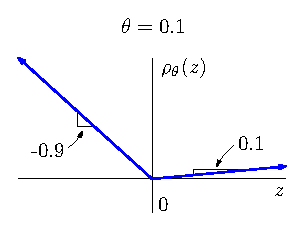
\includegraphics{check-loss-0-1}
  \end{minipage}
  \begin{minipage}[t]{0.33\linewidth}
    \centering
    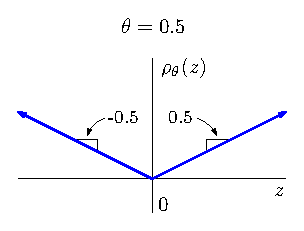
\includegraphics{check-loss-0-5}
  \end{minipage}
  \begin{minipage}[t]{0.33\linewidth}
    \centering
    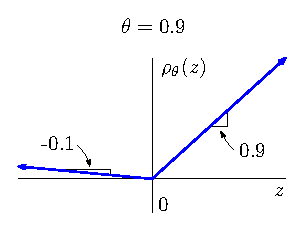
\includegraphics{check-loss-0-9}
  \end{minipage}
  
\end{figure}
Two small examples are provided in Figure \ref{fig:phi-lambda} to further
demonstrate the $\theta$-th quantile classifier and the relationship between the
quantile distances and the difference of the quantile distances.  In these
examples we suppose that $F_0^{-1}(\theta) < F_1^{-1}(\theta)$ at both the 0.25-
and 0.75-th quantile levels, and that $F_1^{-1}(\theta) - F_0^{-1}(\theta)$ is
the same for the two quantile levels.  This is the case for example for
populations that follow $N(0, 1)$ and $N(1, 1)$ distributions.  In the
upper-left plot we show the check loss distance to the populations' 0.25-th
quantiles as a function of input $z$ and denoted as $\Phi_1$ and $\Phi_0$, while
in the bottom-left plot we show the difference of these same check loss
distances, i.e.  $\Lambda = \Phi_1 - \Phi_0$, again as a function of input $z$.
The upper-right and lower right plots also show the check loss distances and
difference between the distances, but instead with respect to the populations'
0.75-th quantiles.  In each of these figures $\tau_{\theta}$ can be seen to
represent the decision rule boundary point, i.e. when $\Lambda = 0$.  We note
that the decision rule boundary is always between $F_{0}^{-1}$ and $F_{1}^{-1}$,
and that when the quantile level is less than 1/2 that $\tau_{\theta}$ is closer
to $F_{1}^{-1}$, and conversely that when the quantile level is greater than 1/2
that $\tau_{\theta}$ is closer to $F_{0}^{-1}$.  Finally, we note that $\Lambda$
is piecewise linear with a slope of $-1$ between $F_{0}^{-1}(\theta)$ and
$F_{1}^{-1}(\theta)$, and is constant otherwise.

Finally, let $Z$ be a random variable with a prior probability $\pi_0$ of being
a member of population $\Pi_0$, and $\pi_1 = 1 - \pi_0$ the prior probability of
being a member of population $\Pi_1$.  Then the probability of correctly
classifying an observed realization of $Z$ by the $\theta$-th quantile
classifier is given by
\begin{equation}
  \label{eq:theoretical-rate}
  \Psi(\theta) =
  \pi_0 \int \ind\Big( \Lambda(z, \theta) > 0 \Big)\, dP_0(z) +
  \pi_1 \int \ind\Big(\Lambda(z, \theta) \leq 0 \Big)\, dP_1(z).
\end{equation}
The expression given in (\ref{eq:theoretical-rate}) has the appealing property
that for the optimal choice of quantile level $\theta$ and under some conditions
that the classification rate is equal to that of the Bayes classifier.  This
result is formally stated in Section \ref{sec:quantile-classifier-optimality} as
Lemma \ref{thm:quantile-classifier-is-bayes}.  We call the quantile classifier
with the optimal quantile level $\theta$ the optimal quantile classifier.  Since
in practice the optimal choice of $\theta$ is unknown, this necessitates the
emprically optimal quantile classifier, which is presented in Section
\ref{sec:empirical-classifier}.


\begin{figure}[ht]
  \caption[cccc]{Example within-class quantile distances and difference in
    quantile distances for two choices of quantiles.}

  \label{fig:phi-lambda}
  \vspace{5mm}
  
  \begin{minipage}[t]{0.49\linewidth}
    \centering
    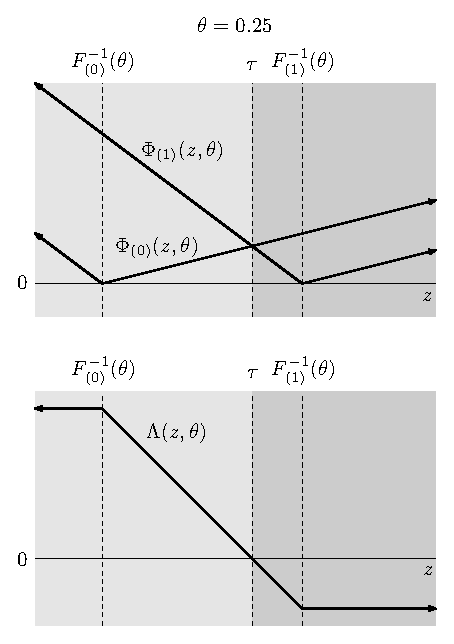
\includegraphics{phi-lambda-0-25}
  \end{minipage}
  \begin{minipage}[t]{0.49\linewidth}
    \centering
    \includegraphics{phi-lambda-0-75}
  \end{minipage}
  
\end{figure}




\subsection{The empirically optimal quantile classifier}
\label{sec:empirical-classifier}

Next we introduce some terminology with which to introduce the sample version of
the optimal quantile classifier.  Let $x_1, \dots, x_m$ be samples from a
population with a probability density on $\mathbb{R}$.  Then we define the
$\theta$-th empirical quantile for the population to be given by any minimizer
of the sample version of equation (\ref{eq:check-loss-min}), defined by
\begin{equation}
  \label{eq:empirical-quantile}
  \hat{F}^{-1} (\theta) = \argmin_q \left\{
    \theta \sum_{ x_{i} > q } |x_{i} - q| ~+~
    (1 - \theta) \sum_{ x_{i} \leq q } |x_{i} - q|
  \right\}.
\end{equation}
It is interesting to note that we can view equation
(\ref{eq:empirical-quantile}) as the solution to a quantile regression problem
introduced in \cite{koenker1978}, where the $x_i$'s correspond to the response
variables, and $q$ is a single regression coefficient corresponding to predictor
data with only an intercept term and no other covariates.  In light of this
fact, we may utilize any of the theory developed in the quantile regression
literature to solve this minimization problem.  However, it turns out that there
is a simple closed-form solution available for this particular special case of
quantile regression, which is presented as Lemma \ref{lem:empirical-quantlev}.

Having defined the $\theta$-th empirical quantile for the population, it follows
that the empirical difference of the quantile distances of a point $z$ to the
population's $\theta$-th quantiles is defined as
\[
  \Lambda_n (z, \theta) = \rho_{\theta}\Big(z - \hat{F}_{1n}^{-1}(\theta)\Big) -
  \rho_{\theta}\Big(z - \hat{F}_{0n}^{-1}(\theta)\Big),
\]
where $\hat{F}_{1n}$ is the estimate of the $\theta$-th quantile level of
population $\Pi_1$ based on the samples in $x_1, \dots, x_n$ that came from
population $\Pi_1$, and similarly for $\hat{F}_{0n}$.  Let $n_0$ and $n_1$
be the number of observations from $\Pi_0$, and $\Pi_1$, respectively.  Then we
further define the observed rate of correct classification for the $\theta$-th
quantile as
\begin{align}
  \begin{split}
    \Psi_n(\theta)
    &= \frac{n_0}{n_0 + n_1} \left[
      \frac{1}{n_0} \sum_{x_i \in \Pi_0}
      \mathbbm{1}\Big( \Lambda_n(x_i, \theta) > 0 \Big)
    \right] +
      \frac{n_1}{n_0 + n_1} \left[
        \frac{1}{n_1} \sum_{x_i \in \Pi_1}
        \mathbbm{1}\Big( \Lambda_n(x_i, \theta) \leq 0 \Big)
      \right] \\[1ex]
    &= \frac{1}{n} \left[
      \sum_{x_i \in \Pi_0} \mathbbm{1}\Big( \Lambda_n(x_i, \theta) > 0 \Big) +
      \sum_{x_i \in \Pi_1} \mathbbm{1}\Big( \Lambda_n(x_i, \theta) \leq 0 \Big)
    \right].
  \end{split}
\end{align}
Finally, define the empirically optimal quantile classifier to be any solution
to the equation
\begin{equation}
  \label{eq:theta-hat}
  \hat{\theta}_n = \argmax_{\theta \in T} \Psi_n(\theta),
\end{equation}
where $T = [\delta, 1 - \delta]$ for some small positive constant $\delta$.  The
restriction of quantile levels to the set $T$ is to guarantee at least one
optimal value of $\theta$ for the theoretical quantile classifier.




\subsection{Optimality and consistency of the quantile classifier}
\label{sec:quantile-classifier-optimality}

With the definitions for the quantile classifier in place, we now provide some
of its properties.  We begin with the fundamental result for the motivation of
the paper, that the quantile classifier achieves the Bayes error rate for the
optimal choice of quantile level.  The following result is due to
\cite{hennig2016}.

\begin{lemma}
  \label{thm:quantile-classifier-is-bayes}
  Consider two populations $\Pi_0$ and $\Pi_1$ with corresponding density
  functions $f_0$ and $f_1$ such that $f_0$ and $f_1$ are nonzero on the same
  domain.  Let $Z$ be a random variable with a prior probability $\pi_0$ of
  being a member of population $\Pi_0$, and $\pi_1 = 1 - \pi_0$ the prior
  probability of being a member of population $\Pi_1$.  Further assume that
  there is a point $z^{*}$ with $\pi_0\, f_0(z^{*}) = \pi_1\, f_1(z^{*})$ so
  that $\pi_0\, f_0(z) < \pi_1\, f_1(z)$ for $z$ on one size of $z^{*}$, and
  $\pi_0\, f_0(z) > \pi_1\, f_1(z)$ on the other side of $z^{*}$.  Then the
  quantile classifier for an observed realization of $Z$ using the optimal
  choice of quantile level achieves the Bayes error rate.
\end{lemma}

Having established the theoretical optimality of the quantile classifier, we now
consider the consistency of the empirical version.  The following result is
essentially a special case of a theorem presented in \cite{hennig2016}.  For
this result, we will need the following assumptions.  Let $\delta$ be a small
positive constant.
\begin{enumerate}[label=\emph{Assumption \arabic*.}, align=left]
\item $F_i^{-1}$ is a continuous function of
  $\theta,~ i=0,1$.
\item $\prob\Big( \Lambda(Z, \theta) = 0 \Big) = 0$ for all
  $\theta \in [\delta, 1 - \delta]$.
\item There is a unique $\tilde{\theta}$ that satisfies $\tilde{\theta} =
  \argmax_{\theta \in T} \Psi(\theta)$.
\end{enumerate}

\begin{lemma}
  \label{lem:univariate-consistency}
  Let $\tilde{\theta}$ be a solution to
  $\tilde{\theta} = \argmax_{\theta \in T} \Psi(\theta)$.  Under Assumptions 1
  and 2, it follows that
  $\Psi(\hat{\theta}_n) \stackrel{p}{\longrightarrow} \Psi(\tilde{\theta})$ with
  $\hat{\theta}_n$ defined in equation (\ref{eq:theta-hat}).  Furthermore, under
  Assumptions 1, 2, and 3, it follows that
  $\hat{\theta}_n \stackrel{p}{\longrightarrow} \tilde{\theta}$.
\end{lemma}

It is worth noting that convergence to the optimal quantile level is based on
the empirically optimal choice for a training data set without the need for
additional training on a validation data set.  Intuitively, this can be
explained by the fact that the model complexity is the same for all of the
possible quantile classifier models, so we do not need to include a model
validation training step to defend against overfitting the model to the data.




\subsection{Decision rule calculation}
\label{sec:empirical-quantile-classifier-results}

So far it has been established that the classification rate of the empirically
optimal quantile classifier converges to the classification rate of the true
optimal quantile classifier.  In this section we investigate the practical
considerations of calculating the empirically optimal quantile classifier.  We
begin by providing an expression for the quantile classifier decision rule
boundary in Lemma \ref{lem:decision-boundary}.

\begin{lemma}
  \label{lem:decision-boundary}
  Assume for the moment that $F_{0}^{-1}(\theta) < F_{1}^{-1}(\theta)$.  Then
  the quantile classifier defined in equation (\ref{eq:quantile-classifier}) can
  be equivalently expressed as follows.
  \begin{equation}
    \label{eq:alt-quantile-classifier-less}
    \text{For an observation $z$, classify to:} \hspace{5mm} \left\{ 
      \begin{array}{lcl}
        \Pi_{0}, & & z ~<~ \theta\, F_{0}^{-1}(\theta) +
                       (1 - \theta)\, F_{1}^{-1}(\theta) \\[1ex]
        % \Pi_{1}, & & z ~=~ \theta F_{(0)}^{-1}(\theta) +
        %                (1 - \theta)\, F_{(1)}^{-1}(\theta) \\[1ex]
        \Pi_{1}, & & \textup{otherwise}
      \end{array} .
    \right.
  \end{equation}
  If on the other hand $F_{0}^{-1}(\theta) > F_{1}^{-1}(\theta)$, then the
  direction of the inequality changes so that we instead classify an observation
  to $\Pi_0$ when
  $z ~>~ \theta\, F_{0}^{-1}(\theta) + (1 - \theta)\, F_{1}^{-1}(\theta)$, and
  to $\Pi_1$ otherwise.
\end{lemma}

It is interesting to note that the decision rule boundary lies on the line
segment between $F_0^{-1}(\theta)$ and $F_1^{-1}(\theta)$, with the location of
the point on the line segment determined by the quantile level.  We saw an
example of this in Figure \ref{fig:phi-lambda} in that for the 0.25-th quantile
level the decision rule boundary was closer to the larger quantile, and for the
0.75-th quantile level the decision rule boundary was closer to the smaller
quantile.

Next, the result given in Lemma \ref{lem:empirical-quantlev} provides an
expression with which to obtain an optimal solution for the empirical quantile
estimator.  

\begin{lemma}
  \label{lem:empirical-quantlev}
  Let $x_1, \dots, x_m$ be points on $\mathbb{R}$.  Then a solution to equation
  (\ref{eq:empirical-quantile}) providing the $\theta$-th empirical quantile for
  $x_1, \dots, x_m$ is given by $\lceil m \theta \rceil$-th largest value of the
  $x_i$.
\end{lemma}

Futhermore, as a consequence of the results of Lemmas
\ref{lem:decision-boundary} and \ref{lem:empirical-quantlev}, the result in
Lemma \ref{lem:decision-rule-time} characterizes the complexity of obtaining the
empirical decision rule boundary for a given dataset.

\begin{lemma}
  \label{lem:decision-rule-time}
  Obtaining the quantile classifier decision rule boundary for a fixed choice of
  quantile level is an $\bigO(n)$ operation.
\end{lemma}




\subsection{Calculating the empirically optimal quantile classifier}
\label{sec:empirically-optimal-algo}

Given the availability of a closed-form expression for the decision rule
boundary at a fixed quantile level, an immediately apparent question is whether
an empirically optimal quantile classifier can be efficiently obtained.
Intuitively, we can sort the data and simply ``slide'' the decision rule
boundary across the range of the data, counting the number of data points for
either class on the correct side of the boundary to find an optimal choice.
Furthermore, since the classification rate doesn't change as we slide the
decision boundary in-between observations, we need only calculate the
classification rate for some countable number of decision boundary choices.

A sketch of the procedure to calculate the empirical classification rate over
the entire space of quantile levels is presented below, and a more detailed
description is provided in the supplementary materials.  The basic idea is that
the quantile estimates $\hat{F}_0^{-1}$ and $\hat{F}_1^{-1}$ are step functions
with respect to the quantile level and with change points occuring on the sets
$\left\{\frac{1}{n_0}, \dots, \frac{n_o - 1}{n_0}\right\}$ and
$\left\{\frac{1}{n_1}, \dots, \frac{n_1 - 1}{n_1}\right\}$, respectively.  Thus
for intervals not containing any of these points except as endpoints, the
quantile estimates are fixed and the interval can be mapped to a contiguous
interval of decision rule boundaries.  Within these decision rule boundary
intervals we can further partition a given interval into sub-intervals that each
has a constant empirical classification rate by letting the partition boundaries
be defined by any data points contained in the interval.  Thus by counting the
number of data points from each class on either side of the decision boundary
for every sub-interval we obtain the empirical classification rate over the
entire quantile level space.  A high-level version of the algorithm is presented
as Algorithm \ref{alg:empirically-optimal-classifier}, and a result for the
algorithm complexity is presented as Proposition
\ref{lem:optimal-quantile-time}.

An illustrative example for a small data set is presented as Figure
\ref{fig:empirical-classification-rate} showing the decision rule boundary and
corresponding classification rate as a function of the quantile level.  A data
set for class 0 with 7 observations was sampled from independent $N(0, 1)$
distributions yielding the values
$-0.96,\allowbreak -0.78,\allowbreak -0.46,\allowbreak -0.10,\allowbreak
0.24,\allowbreak 0.98,\allowbreak 1.61$, and a data set for class 1 with 5
observations was sampled from independent $N(1, 1)$ distributions yielding the
values
$-0.60,\allowbreak 0.37,\allowbreak 0.64,\allowbreak 1.37,\allowbreak 1.78$.
These values are shown as the horizontal lines in the top panel, along with the
decision rule boundaries corresponding to this data which are displayed as the
diagonal blue lines.  The dashed vertical lines represent the quantile levels at
which the quantile estimates change for at least one of the classes.  In the
bottom panel the number of correctly classified observations out of a possible
12 observations is plotted as a function of the quantile level.  From this
figure we see that the classification rate of the quantile classifier is
constant for the intervals between the quantile estimate change points except
when the set of corresponding decision rule boundary values includes values in
the data.  When this is the case the intervals can be further divided into
sub-intervals with a constant classification rate.  For this particular example
the theoretically optimal quantile level is 0.5, which is indeed one of the
empirically optimal quantile levels.

One issue that has yet to be addressed that is evident in this example is how to
choose a quantile level based on a training data set when there is more than one
empirically optimal value.  When this is the case, as it typically is, we find
that selecting the value closest to the median works well in many settings.  One
argument for this choice is that the median is the optimal choice of quantile
level for two classes with symmetric distributions that differ only by a
location shift.  While this scenario may not hold in many settings, it still
offers in some sense a conservative rule for what is hopefully a small set of
empirically quantile levels from which to choose.

\begin{figure}[p]
  \caption[Example empirical classification rate]{Illustrative plot of the
    empirical classification rate for a toy example.  An example data set is
    shown with 7 values from class $\Pi_0$ and 5 values from class $\Pi_1$. }
  \label{fig:empirical-classification-rate}
  \centering
  \vspace{5mm}

  \includegraphics[width=1\textwidth]{emp_quant_example}
\end{figure}




\begin{algorithm}[ht]
  \caption{Calculating the empirically optimal quantile classifier}
  \label{alg:empirically-optimal-classifier}
  \DontPrintSemicolon
  \BlankLine
  \SetKwInOut{Input}{Data}
  \Input{$v_1, \dots, v_{n_0}$ from $\Pi_0$ and $w_1, \dots, w_{n_1}$ in
    $\Pi_1$}


  Sort $v_1, \dots, v_{n_0}, w_1, \dots, w_{n_1}$ and denote the unique values
  as $x_1, \dots, x_r$
  
  Produce a sorted set of quantile levels given by
  $ \Theta = \Big\{ 0 \Big\} \bigcup \left\{ \frac{k}{n_0}: 1 \leq k \leq n_0
  \right\} \bigcup \left\{ \frac{k}{n_1}: 1 \leq k \leq n_1 \right\} $

  \BlankLine

  \For{$i$ in 2 to $|\Theta|$}{
    
    \BlankLine
    
    calculate $\hat{F}_V^{-1}(\theta_i)$ and $\hat{F}_W^{-1}(\theta_i)$, and
    find \vspace{-0mm}
    \begin{equation*}
      a = \min \Big\{ \hat{F}_0^{-1}(\theta_i),~ \hat{F}_1^{-1}(\theta_i) \Big\}
      \hspace{5mm} \text{and} \hspace{5mm}
      b = \max \Big\{ \hat{F}_0^{-1}(\theta_i),~ \hat{F}_1^{-1}(\theta_i) \Big\}
    \end{equation*}
    \vspace{-5mm}
    
    calculate the interval
    \vspace{-0mm}
    \[
      G_i = \Big[
      \theta_i\, a + (1 - \theta_i)\, b,
      \hspace{3mm}
      \theta_{i-1}\, a + (1 - \theta_{i-1})\, b\,
      \Big) = \big[x_{\scriptscriptstyle\text{low}},\,
      x_{\scriptscriptstyle\text{high}}\big)
    \]

    partition
    $\big[x_{\scriptscriptstyle\text{low}},\,
    x_{\scriptscriptstyle\text{high}}\big)$ where the partition boundaries are
    given by any $x_i$ in the interval, and calculate the classification rate
    for each sub-interval
    
  }
\end{algorithm}


\begin{proposition}
  \label{lem:optimal-quantile-time}
  The decision rule for the empirically optimal quantile classifier can be
  obtained in $\mathcal{O}(n^2)$ time.
\end{proposition}

It remains an open question as to whether the bound obtained in Proposition
\ref{lem:optimal-quantile-time} is actually achievable.  In practice, for both
simulated and real data we typically see less than $n$ total intervals that need
to be considered in the outer and inner loops, so when this is the case the
algorithm runs in $\mathcal{O}(n \log n)$ time.  As an alternative, we can
approximate the empirically optimal quantile classifier by simply calculating
the empirical classification rate over a fine grid of quantile levels, which
reduces the complexity to an $\mathcal{O}(Kn)$ operation where $K$ is the number
of points in the grid.  This complexity is the case because each choice of
quantile level requires calculating the decision rule boundary by finding the
$k_0$-th and $k_1$-th largest value of each class for the appropriate values of
$k_0$ and $k_1$, and then counting the number of observations on the correct
side of the boundary, each of which is an $\mathcal{O}(n)$ operation.




%%% Local Variables:
%%% mode: latex
%%% TeX-master: "cqc_paper"
%%% End:
